%% bare_jrnl.tex
%% V1.4b
%% 2015/08/26
%% by Michael Shell
%% see http://www.michaelshell.org/
%% for current contact information.
%%
%% This is a skeleton file demonstrating the use of IEEEtran.cls
%% (requires IEEEtran.cls version 1.8b or later) with an IEEE
%% journal paper.
%%
%% Support sites:
%% http://www.michaelshell.org/tex/ieeetran/
%% http://www.ctan.org/pkg/ieeetran
%% and
%% http://www.ieee.org/

%%*************************************************************************
%% Legal Notice:
%% This code is offered as-is without any warranty either expressed or
%% implied; without even the implied warranty of MERCHANTABILITY or
%% FITNESS FOR A PARTICULAR PURPOSE! 
%% User assumes all risk.
%% In no event shall the IEEE or any contributor to this code be liable for
%% any damages or losses, including, but not limited to, incidental,
%% consequential, or any other damages, resulting from the use or misuse
%% of any information contained here.
%%
%% All comments are the opinions of their respective authors and are not
%% necessarily endorsed by the IEEE.
%%
%% This work is distributed under the LaTeX Project Public License (LPPL)
%% ( http://www.latex-project.org/ ) version 1.3, and may be freely used,
%% distributed and modified. A copy of the LPPL, version 1.3, is included
%% in the base LaTeX documentation of all distributions of LaTeX released
%% 2003/12/01 or later.
%% Retain all contribution notices and credits.
%% ** Modified files should be clearly indicated as such, including  **
%% ** renaming them and changing author support contact information. **
%%*************************************************************************


% *** Authors should verify (and, if needed, correct) their LaTeX system  ***
% *** with the testflow diagnostic prior to trusting their LaTeX platform ***
% *** with production work. The IEEE's font choices and paper sizes can   ***
% *** trigger bugs that do not appear when using other class files.       ***                          ***
% The testflow support page is at:
% http://www.michaelshell.org/tex/testflow/



\documentclass[journal]{IEEEtran}
%
\usepackage{graphicx}
\usepackage{caption,setspace}
\usepackage{amsmath}
\usepackage[ruled,vlined]{algorithm2e}

\usepackage{tabularx}
\usepackage{hyperref}

\usepackage{subcaption}
% If IEEEtran.cls has not been installed into the LaTeX system files,
% manually specify the path to it like:
% \documentclass[journal]{../sty/IEEEtran}





% Some very useful LaTeX packages include:
% (uncomment the ones you want to load)


% *** MISC UTILITY PACKAGES ***
%
%\usepackage{ifpdf}
% Heiko Oberdiek's ifpdf.sty is very useful if you need conditional
% compilation based on whether the output is pdf or dvi.
% usage:
% \ifpdf
%   % pdf code
% \else
%   % dvi code
% \fi
% The latest version of ifpdf.sty can be obtained from:
% http://www.ctan.org/pkg/ifpdf
% Also, note that IEEEtran.cls V1.7 and later provides a builtin
% \ifCLASSINFOpdf conditional that works the same way.
% When switching from latex to pdflatex and vice-versa, the compiler may
% have to be run twice to clear warning/error messages.






% *** CITATION PACKAGES ***
%
%\usepackage{cite}
% cite.sty was written by Donald Arseneau
% V1.6 and later of IEEEtran pre-defines the format of the cite.sty package
% \cite{} output to follow that of the IEEE. Loading the cite package will
% result in citation numbers being automatically sorted and properly
% "compressed/ranged". e.g., [1], [9], [2], [7], [5], [6] without using
% cite.sty will become [1], [2], [5]--[7], [9] using cite.sty. cite.sty's
% \cite will automatically add leading space, if needed. Use cite.sty's
% noadjust option (cite.sty V3.8 and later) if you want to turn this off
% such as if a citation ever needs to be enclosed in parenthesis.
% cite.sty is already installed on most LaTeX systems. Be sure and use
% version 5.0 (2009-03-20) and later if using hyperref.sty.
% The latest version can be obtained at:
% http://www.ctan.org/pkg/cite
% The documentation is contained in the cite.sty file itself.






% *** GRAPHICS RELATED PACKAGES ***
%
\ifCLASSINFOpdf
  % \usepackage[pdftex]{graphicx}
  % declare the path(s) where your graphic files are
  % \graphicspath{{../pdf/}{../jpeg/}}
  % and their extensions so you won't have to specify these with
  % every instance of \includegraphics
  % \DeclareGraphicsExtensions{.pdf,.jpeg,.png}
\else
  % or other class option (dvipsone, dvipdf, if not using dvips). graphicx
  % will default to the driver specified in the system graphics.cfg if no
  % driver is specified.
  % \usepackage[dvips]{graphicx}
  % declare the path(s) where your graphic files are
  % \graphicspath{{../eps/}}
  % and their extensions so you won't have to specify these with
  % every instance of \includegraphics
  % \DeclareGraphicsExtensions{.eps}
\fi
% graphicx was written by David Carlisle and Sebastian Rahtz. It is
% required if you want graphics, photos, etc. graphicx.sty is already
% installed on most LaTeX systems. The latest version and documentation
% can be obtained at: 
% http://www.ctan.org/pkg/graphicx
% Another good source of documentation is "Using Imported Graphics in
% LaTeX2e" by Keith Reckdahl which can be found at:
% http://www.ctan.org/pkg/epslatex
%
% latex, and pdflatex in dvi mode, support graphics in encapsulated
% postscript (.eps) format. pdflatex in pdf mode supports graphics
% in .pdf, .jpeg, .png and .mps (metapost) formats. Users should ensure
% that all non-photo figures use a vector format (.eps, .pdf, .mps) and
% not a bitmapped formats (.jpeg, .png). The IEEE frowns on bitmapped formats
% which can result in "jaggedy"/blurry rendering of lines and letters as
% well as large increases in file sizes.
%
% You can find documentation about the pdfTeX application at:
% http://www.tug.org/applications/pdftex





% *** MATH PACKAGES ***
%
%\usepackage{amsmath}
% A popular package from the American Mathematical Society that provides
% many useful and powerful commands for dealing with mathematics.
%
% Note that the amsmath package sets \interdisplaylinepenalty to 10000
% thus preventing page breaks from occurring within multiline equations. Use:
%\interdisplaylinepenalty=2500
% after loading amsmath to restore such page breaks as IEEEtran.cls normally
% does. amsmath.sty is already installed on most LaTeX systems. The latest
% version and documentation can be obtained at:
% http://www.ctan.org/pkg/amsmath





% *** SPECIALIZED LIST PACKAGES ***
%
%\usepackage{algorithmic}
% algorithmic.sty was written by Peter Williams and Rogerio Brito.
% This package provides an algorithmic environment fo describing algorithms.
% You can use the algorithmic environment in-text or within a figure
% environment to provide for a floating algorithm. Do NOT use the algorithm
% floating environment provided by algorithm.sty (by the same authors) or
% algorithm2e.sty (by Christophe Fiorio) as the IEEE does not use dedicated
% algorithm float types and packages that provide these will not provide
% correct IEEE style captions. The latest version and documentation of
% algorithmic.sty can be obtained at:
% http://www.ctan.org/pkg/algorithms
% Also of interest may be the (relatively newer and more customizable)
% algorithmicx.sty package by Szasz Janos:
% http://www.ctan.org/pkg/algorithmicx




% *** ALIGNMENT PACKAGES ***
%
%\usepackage{array}
% Frank Mittelbach's and David Carlisle's array.sty patches and improves
% the standard LaTeX2e array and tabular environments to provide better
% appearance and additional user controls. As the default LaTeX2e table
% generation code is lacking to the point of almost being broken with
% respect to the quality of the end results, all users are strongly
% advised to use an enhanced (at the very least that provided by array.sty)
% set of table tools. array.sty is already installed on most systems. The
% latest version and documentation can be obtained at:
% http://www.ctan.org/pkg/array


% IEEEtran contains the IEEEeqnarray family of commands that can be used to
% generate multiline equations as well as matrices, tables, etc., of high
% quality.




% *** SUBFIGURE PACKAGES ***
%\ifCLASSOPTIONcompsoc
%  \usepackage[caption=false,font=normalsize,labelfont=sf,textfont=sf]{subfig}
%\else
%  \usepackage[caption=false,font=footnotesize]{subfig}
%\fi
% subfig.sty, written by Steven Douglas Cochran, is the modern replacement
% for subfigure.sty, the latter of which is no longer maintained and is
% incompatible with some LaTeX packages including fixltx2e. However,
% subfig.sty requires and automatically loads Axel Sommerfeldt's caption.sty
% which will override IEEEtran.cls' handling of captions and this will result
% in non-IEEE style figure/table captions. To prevent this problem, be sure
% and invoke subfig.sty's "caption=false" package option (available since
% subfig.sty version 1.3, 2005/06/28) as this is will preserve IEEEtran.cls
% handling of captions.
% Note that the Computer Society format requires a larger sans serif font
% than the serif footnote size font used in traditional IEEE formatting
% and thus the need to invoke different subfig.sty package options depending
% on whether compsoc mode has been enabled.
%
% The latest version and documentation of subfig.sty can be obtained at:
% http://www.ctan.org/pkg/subfig




% *** FLOAT PACKAGES ***
%
%\usepackage{fixltx2e}
% fixltx2e, the successor to the earlier fix2col.sty, was written by
% Frank Mittelbach and David Carlisle. This package corrects a few problems
% in the LaTeX2e kernel, the most notable of which is that in current
% LaTeX2e releases, the ordering of single and double column floats is not
% guaranteed to be preserved. Thus, an unpatched LaTeX2e can allow a
% single column figure to be placed prior to an earlier double column
% figure.
% Be aware that LaTeX2e kernels dated 2015 and later have fixltx2e.sty's
% corrections already built into the system in which case a warning will
% be issued if an attempt is made to load fixltx2e.sty as it is no longer
% needed.
% The latest version and documentation can be found at:
% http://www.ctan.org/pkg/fixltx2e


%\usepackage{stfloats}
% stfloats.sty was written by Sigitas Tolusis. This package gives LaTeX2e
% the ability to do double column floats at the bottom of the page as well
% as the top. (e.g., "\begin{figure*}[!b]" is not normally possible in
% LaTeX2e). It also provides a command:
%\fnbelowfloat
% to enable the placement of footnotes below bottom floats (the standard
% LaTeX2e kernel puts them above bottom floats). This is an invasive package
% which rewrites many portions of the LaTeX2e float routines. It may not work
% with other packages that modify the LaTeX2e float routines. The latest
% version and documentation can be obtained at:
% http://www.ctan.org/pkg/stfloats
% Do not use the stfloats baselinefloat ability as the IEEE does not allow
% \baselineskip to stretch. Authors submitting work to the IEEE should note
% that the IEEE rarely uses double column equations and that authors should try
% to avoid such use. Do not be tempted to use the cuted.sty or midfloat.sty
% packages (also by Sigitas Tolusis) as the IEEE does not format its papers in
% such ways.
% Do not attempt to use stfloats with fixltx2e as they are incompatible.
% Instead, use Morten Hogholm'a dblfloatfix which combines the features
% of both fixltx2e and stfloats:
%
% \usepackage{dblfloatfix}
% The latest version can be found at:
% http://www.ctan.org/pkg/dblfloatfix




%\ifCLASSOPTIONcaptionsoff
%  \usepackage[nomarkers]{endfloat}
% \let\MYoriglatexcaption\caption
% \renewcommand{\caption}[2][\relax]{\MYoriglatexcaption[#2]{#2}}
%\fi
% endfloat.sty was written by James Darrell McCauley, Jeff Goldberg and 
% Axel Sommerfeldt. This package may be useful when used in conjunction with 
% IEEEtran.cls'  captionsoff option. Some IEEE journals/societies require that
% submissions have lists of figures/tables at the end of the paper and that
% figures/tables without any captions are placed on a page by themselves at
% the end of the document. If needed, the draftcls IEEEtran class option or
% \CLASSINPUTbaselinestretch interface can be used to increase the line
% spacing as well. Be sure and use the nomarkers option of endfloat to
% prevent endfloat from "marking" where the figures would have been placed
% in the text. The two hack lines of code above are a slight modification of
% that suggested by in the endfloat docs (section 8.4.1) to ensure that
% the full captions always appear in the list of figures/tables - even if
% the user used the short optional argument of \caption[]{}.
% IEEE papers do not typically make use of \caption[]'s optional argument,
% so this should not be an issue. A similar trick can be used to disable
% captions of packages such as subfig.sty that lack options to turn off
% the subcaptions:
% For subfig.sty:
% \let\MYorigsubfloat\subfloat
% \renewcommand{\subfloat}[2][\relax]{\MYorigsubfloat[]{#2}}
% However, the above trick will not work if both optional arguments of
% the \subfloat command are used. Furthermore, there needs to be a
% description of each subfigure *somewhere* and endfloat does not add
% subfigure captions to its list of figures. Thus, the best approach is to
% avoid the use of subfigure captions (many IEEE journals avoid them anyway)
% and instead reference/explain all the subfigures within the main caption.
% The latest version of endfloat.sty and its documentation can obtained at:
% http://www.ctan.org/pkg/endfloat
%
% The IEEEtran \ifCLASSOPTIONcaptionsoff conditional can also be used
% later in the document, say, to conditionally put the References on a 
% page by themselves.




% *** PDF, URL AND HYPERLINK PACKAGES ***
%
%\usepackage{url}
% url.sty was written by Donald Arseneau. It provides better support for
% handling and breaking URLs. url.sty is already installed on most LaTeX
% systems. The latest version and documentation can be obtained at:
% http://www.ctan.org/pkg/url
% Basically, \url{my_url_here}.




% *** Do not adjust lengths that control margins, column widths, etc. ***
% *** Do not use packages that alter fonts (such as pslatex).         ***
% There should be no need to do such things with IEEEtran.cls V1.6 and later.
% (Unless specifically asked to do so by the journal or conference you plan
% to submit to, of course. )


% correct bad hyphenation here
\hyphenation{op-tical net-works semi-conduc-tor}


\begin{document}
%
% paper title
% Titles are generally capitalized except for words such as a, an, and, as,
% at, but, by, for, in, nor, of, on, or, the, to and up, which are usually
% not capitalized unless they are the first or last word of the title.
% Linebreaks \\ can be used within to get better formatting as desired.
% Do not put math or special symbols in the title.
\title{Comparison of Adaptive Bitrate Algorithms for Multi-user DASH Video Streaming}
%
%
% author names and IEEE memberships
% note positions of commas and nonbreaking spaces ( ~ ) LaTeX will not break
% a structure at a ~ so this keeps an author's name from being broken across
% two lines.
% use \thanks{} to gain access to the first footnote area
% a separate \thanks must be used for each paragraph as LaTeX2e's \thanks
% was not built to handle multiple paragraphs
%

\author{Hai-Dang Nguyen}
       % <-this % stops a space
% \thanks{M. Shell was with the Department
% of Electrical and Computer Engineering, Georgia Institute of Technology, Atlanta,
% GA, 30332 USA e-mail: (see http://www.michaelshell.org/contact.html).}% <-this % stops a space
% \thanks{J. Doe and J. Doe are with Anonymous University.}% <-this % stops a space
% \thanks{Manuscript received April 19, 2005; revised August 26, 2015.}


% note the % following the last \IEEEmembership and also \thanks - 
% these prevent an unwanted space from occurring between the last author name
% and the end of the author line. i.e., if you had this:
% 
% \author{....lastname \thanks{...} \thanks{...} }
%                     ^------------^------------^----Do not want these spaces!
%
% a space would be appended to the last name and could cause every name on that
% line to be shifted left slightly. This is one of those "LaTeX things". For
% instance, "\textbf{A} \textbf{B}" will typeset as "A B" not "AB". To get
% "AB" then you have to do: "\textbf{A}\textbf{B}"
% \thanks is no different in this regard, so shield the last } of each \thanks
% that ends a line with a % and do not let a space in before the next \thanks.
% Spaces after \IEEEmembership other than the last one are OK (and needed) as
% you are supposed to have spaces between the names. For what it is worth,
% this is a minor point as most people would not even notice if the said evil
% space somehow managed to creep in.



% The paper headers
\markboth{Joint project - HaiDang Nguyen}%
{Shell \MakeLowercase{\textit{et al.}}: Bare Demo of IEEEtran.cls for IEEE Journals}
% The only time the second header will appear is for the odd numbered pages
% after the title page when using the twoside option.
% 
% *** Note that you probably will NOT want to include the author's ***
% *** name in the headers of peer review papers.                   ***
% You can use \ifCLASSOPTIONpeerreview for conditional compilation here if
% you desire.




% If you want to put a publisher's ID mark on the page you can do it like
% this:
%\IEEEpubid{0000--0000/00\$00.00~\copyright~2015 IEEE}
% Remember, if you use this you must call \IEEEpubidadjcol in the second
% column for its text to clear the IEEEpubid mark.



% use for special paper notices
%\IEEEspecialpapernotice{(Invited Paper)}




% make the title area
\maketitle

% As a general rule, do not put math, special symbols or citations
% in the abstract or keywords.
\begin{abstract}
Dynamic Adaptive Streaming over HTTP (DASH) has currently become a de facto standard for streaming video over the Internet. It contributes towards to leveraging the network friendliness of TCP protocol with firewall and bandwidth sharing. Further more, splitting video in multiple fix-duration segments and pre-encoding them in multiple quality levels introduce a flexible way for bitrate adaptation in various network conditions. 
\par
Recently, a number of Adaptation BitRate (ABR) algorithms have been proposed; most of them, however, was simply evaluated in  single-client cases. In practice, a network system may consist of multiple users, which compete for a bottleneck link. In such scenarios, clients may exhibit un-predicted behaviours, which can cause the fluctuation of perceived bandwidth even when network conditions remain unchanged. In this work, we indicate several biases among clients in multi-user scenarios. We also give a look inside state-of-the-art ABR algorithms and evaluate their performance in multi-user cases in terms of stability, efficiency and fairness. Finally, some improvements was introduced to achieve a better trade-off between aforementioned performance metrics.  
\end{abstract}

% Note that keywords are not normally used for peerreview papers.
\begin{IEEEkeywords}
Bitrate adaptation; HAS; DASH; adaptive video
streaming; ABR schemes.
\end{IEEEkeywords}






% For peer review papers, you can put extra information on the cover
% page as needed:
% \ifCLASSOPTIONpeerreview
% \begin{center} \bfseries EDICS Category: 3-BBND \end{center}
% \fi
%
% For peerreview papers, this IEEEtran command inserts a page break and
% creates the second title. It will be ignored for other modes.
\IEEEpeerreviewmaketitle



\section{Introduction}
% The very first letter is a 2 line initial drop letter followed
% by the rest of the first word in caps.
% 
% form to use if the first word consists of a single letter:
% \IEEEPARstart{A}{demo} file is ....
% 
% form to use if you need the single drop letter followed by
% normal text (unknown if ever used by the IEEE):
% \IEEEPARstart{A}{}demo file is ....
% 
% Some journals put the first two words in caps:
% \IEEEPARstart{T}{his demo} file is ....
% 
% Here we have the typical use of a "T" for an initial drop letter
% and "HIS" in caps to complete the first word.
\IEEEPARstart{R}{ecently}, HTTP streaming has become cost-effective method for multimedia delivery over the Internet \cite{thang}. Due to the bandwidth fluctuation nature of TCP protocol \cite{bandwidth fluc}, which is the underlying layer of HTTP, one of the most important requirements for any streaming systems is bitrate adaptability. To serve for that purpose, a video is chunked into multiple segments, which uniformly last for a fixed duration. A video segment, in turn, is encoded in multiple representations (versions) that differ in bitrate or resolution. A metadata file is also generated to contain characteristics of representations. In a streaming session, A client first fetches the metadata file in order to get information about the video and its segments. An ABR algorithm, which is installed in client side, then decides which video representation should be requested at each time step based on current network conditions or terminal capabilities \cite{general HTTP}. 
\par Numerous ABR algorithms have been proposed to be implemented in client side. They are clustered in three categories: bandwidth-based, buffer-based and mixed adaptation \cite{ABR cats}. Bandwidth-based adaptation makes representation decisions based on its measured bandwidth, which can be calculated as the size of a fetched video segment divided by the its download time. This type of adaption is strongly influenced by bandwidth fluctuation. Meanwhile, buffer-based adaptive algorithms uses the client's buffer occupancy to select the appropriate version of the next segment.  They can absorb short-term oscillations of bandwidth to achieve better bitrate stability. Finally, mixed adaptation makes bitrate selections based on the combination of network conditions and buffer occupancy.  
\par In multi-user scenarios, the competition between clients and the discrete nature of bitrate representations lead to the difficulty in precisely measuring the fair-shared bandwidth \cite{PANDA}. Several methods have been proposed to address this problem \cite{PANDA} \cite{FESTIVE}; however, their bitrate selections are simply based on bandwidth-based adaptation. Meanwhile, buffer-based algorithms \cite{BBA} \cite{BOLA}, which outperform bandwidth-based ones in in terms of efficiency and stability, have not yet evaluated in multi-user scenarios. In this work, we make comparison between the aforementioned adaptive algorithms in a network of multiple clients. We also propose a new algorithm with some improvements in order to achieve better trade-off between performance metrics.  
\par The paper is organized as follow. Section II gives some backgrounds on HTTP Adaptive Streaming. Section III provides related work to give brief review of adaptation methods. Our proposed improvements on state-of-the-art algorithms are detailed in Section IV. Comparisons between algorithms are discussed in Section V. Section VI concludes the paper. 
% You must have at least 2 lines in the paragraph with the drop letter
% (should never be an issue)
\section {Background}
\subsection{HTTP Adaptive Streaming System}
The system architecture of a DASH system is shown in Figure \ref{DASH sys}. At server side, a video content is encoded in multiple versions with different birate levels. Each version then is split into temporal segments. In a streaming session, at first, the client sends a HTTP request to the server in order to obtain metadata file, which contains the information of all video representations (alternatives or versions). A rate adaptation logic at client side, where a ABR algorithm is installed, decides the next segment's bitrate based on several criteria such as measured bandwidth and buffer occupancy at each time step. The video segments are then delivered from the server to the client via a sequence of request-response transactions \cite{thang}. Once a video segment is decoded completely in the client, it will be stored in the client's buffer before being played out.
\par Several factors may impact on Quality of Experience (QoE) in HTTP Streaming. Average bitrate is one of  influence factors \cite{Avg rate}. Authors in \cite{QoE calcu} also indicate that QoE is strongly influenced by the frequency and duration of buffer depletion, which causes playout freezes. Besides, the sudden drop of video bitrate causes adverse impacts on user's experience. \cite{decrease rate}. 
\begin{figure}[!h]
\centering
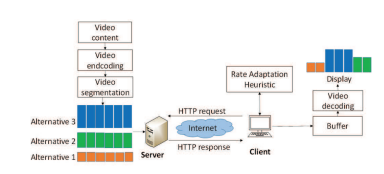
\includegraphics[width=0.5\textwidth]{images/System.PNG}
\captionsetup{justification=centering}
\caption{DASH system architecture.}
\label{DASH sys}
\end{figure}
\subsection{System Model}
A video is chopped into temporal segments of fixed duration $\tau$
seconds. Each segment has been pre-encoded at L video
bitrates, all stored at the server. Denote by $R := {R_1, ..., R_L}$
the set of available video bitrates, with $0 < R_l < R_m$ for
$l < m$.
\par At the beginning of each download step n, a rate adaptation
algorithm will:
\begin{itemize}
	\item Selects the video bitrate of the next segment to be
	downloaded, $r[n] \in R$.
	\item Specifies how much time to give for the current download, until the next download request (i.e., the inter-request time), $\hat{T}[n]$.
\end{itemize}
\par Let $\tilde{T}[n]$ be
the download duration. The next download step starts after the duration of $T[n]$, which is calculated as follow:
\begin{equation}
T[n]=\max(\hat{T}[n],\tilde{T}[n])
\end{equation}
That is if the download duration $\tilde{T}[n]$ shorter than target delay $\hat{T}[n]$, the client have to wait $\hat{T}[n]-\tilde{T}[n]$ until the next download. Figure \ref{Download} illustrates the downloading process in two scenarios. At the beginning of each downloading time step, the scheduled duration $\hat{T}[n]$ and selected bitrate $r[n]$ are updated. In Scenario A, when the segment is downloaded in a duration $\tilde{T}[n]$ shorter than the scheduled duration $\hat{T}[n]$, then the client have to wait until the next time step to take new decisions. Otherwise, in the Scenario B, if the download time is longer than expected, then the client will start downloading next segment immediately.
\begin{figure}[!h]
\centering
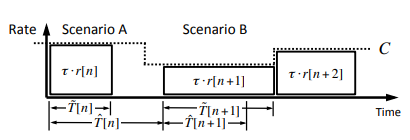
\includegraphics[width=0.5\textwidth]{images/Download.PNG}
\captionsetup{justification=centering}
\caption{Segment downloading process.}
\label{Download}
\end{figure}

\par Once the client has already received the whole segment data, it can measure the network bandwidth $\hat{x[n]}$ as data size divided by download time: 
\begin{equation}
\hat{x}[n]=\dfrac{r[n]\times\tau}{\tilde{T}[n]}
\label{Bandwidth}
\end{equation}
where $x[n]$ is selected bitrate at time step n.
\par 
The buffer occupancy in video streaming is calculated in second other than data size. Assume that the client plays out the video segments at nominal speed, i.e, if a video segment lasts for $\tau$ seconds, the client takes exactly $\tau$ seconds to completely play out it. At each downloading time step $n$, the client receives one more segment of $\tau$ seconds but also consumes $T[n]$ seconds of video compared to last time step $n-1$. Therefore, the buffer occupancy update is formulated as follow:
\begin{equation}
B[n]=\max(0,B[n-1]+\tau-T[n])
\end{equation}
The maximum operation here indicates that the buffer occupancy cannot be negative.
\section{Related work}
\subsection{ABR in multi-user scenarios}
Client-based adaptive bitrate algorithms can be divided into three categories based on the the signal they use to decide the next segment's bitrate: bandwidth-based, buffer-based and mixed adaptation \cite{ABR cats}. Follow \cite{PANDA}, a algorithm should consist of two parts: \begin{itemize}
    \item Measure the next segment bitrate.
    \item Schedule the request for the next video segment.
\end{itemize}
\par While a simple rate adaptation algorithm works fairly with a single client, multiple clients competing a bottleneck link could cause undesirable problems \cite{FESTIVE}. There are two sources of bias in multi-user case. Firstly, with periodic request intervals, the initial condition can cause the unfairness in bandwidth allocation. Secondly, a client requesting higher bitrate can estimate higher bandwidth. This is because there are points that it occupy the bottleneck link alone, and it can consume whole network resource \cite{FESTIVE}. The explanation of such biases is detailed below. 
\par There are two popular options for scheduling: immediate download and periodic download \cite{FESTIVE}. For the first option, the client will download the next chunk immediately after the previous chunk has been downloaded completely. Greedily downloading the low bitrate chunks will ramp-up buffer quickly and cause the buffer overflow. Furthermore, in live streaming, the next chunk cannot be available immediately. In the second option, the chunks is downloaded periodically, so that the buffer is remained at optimal level. The issue with this approach is illustrated in the Figure \ref{ini bias}. Suppose that the players A, B and C compete for a bottleneck link. Players B and C request periodically at even seconds while player A requests at odd seconds. Obviously, players B and C must compete to each other and observe only half of bandwidth while player A is able to use the whole bandwidth. In other words, the initial condition can cause the unfairness in bandwidth allocation.
\begin{figure}[!h]
	\centering
	
	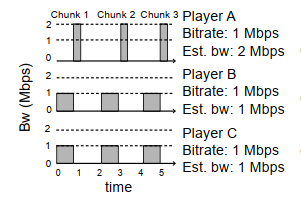
\includegraphics[width=0.5\textwidth]{images/IniBias.PNG}
	
	
	
	\caption{Initial condition bias}
	\label {ini bias}
	
\end{figure}
\par The second type of bias is illustrated in Figure \ref{bitrate bias}. In this case, player A requests higher bitrate compared to player B and C. It can be seen that there are time instants where player A uses the whole bandwidth while this is not the case for the others. Thus, player A will estimate bandwidth higher than players B and C. In other words, players currently opting higher bitrate will perceive higher bandwidth. 
\begin{figure}[!h]
	\centering
	
	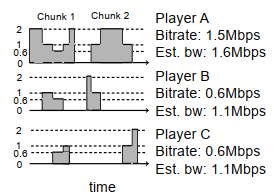
\includegraphics[width=0.5\textwidth]{images/bitrateBias.PNG}
	
	
	
	\caption{Bitrate selection bias}
	\label {bitrate bias}
	
\end{figure} 
\par Follow \cite{PANDA}, in multi-user case, a robust adaptive algorithm must achieve three following goals:
\begin{itemize}
	\item Fairness: Clients competing a bottleneck link will eventually converge to an equitable network resource.  
	\item Efficiency: Clients must choose the highest bitrate as possible to maximize bandwidth usage.
	\item Stability: Clients should avoid the unnecessary bitrate switches as it causes annoyance for users.
\end{itemize}
The following subsections give a look inside state-of-the-art ABR algorithms. The explanation of notions used in algorithms is detailed in Table \ref{notions}.
\begin{table}[]
    \centering
  
    \caption{Notions used in algorithms}
    \label{notions}
    
	\begin{tabularx}{0.5\textwidth}{|l|X|} 
		\hline
		Notions & Explanation  \\ [0.5ex] 
		\hline\hline
		$\tau$ & Segment duration  \\ 
		\hline
		$r[n]$ & Selected bitrate for segment at time step n  \\
		\hline
		 $\hat{x}[n]$& Estimated bandwidth for segment at time step n \\
		\hline
		$\tilde{x}[n]$ & Actual bandwidth of segment at time step n  \\
		\hline
		$R$ & Set of bitrate $R=\{R_1, R_2,...,R_L\}$  \\ 
		\hline
		$T[n]$ & Actual inter-request time of segment at time step n \\  
		\hline
			$\hat{T}[n]$ & Scheduled inter-request time of video segment at time step n \\
			\hline
			$\tilde{T}[n]$ & Download duration of video segment at time step n \\
			\hline
			$B[n]$ & Buffer level after completely downloading of segment at time step n (in seconds) \\
			\hline
			$b[n] = \cfrac{B[n]}{\tau}$ & Buffer level after completely downloading of segment at time step n (in number of segments) \\
			\hline
			$B_{min}/B_{max}$ & Minimum/Maximum client buffer duration \\
			\hline
			$w$ & Probing additive increase bitrate \\
			\hline
			$k$ & Probing convergence rate \\
			\hline
			$\alpha$ & Smoothing convergence rate\\
			\hline
			$\beta$ & Buffer convergence rate\\
			\hline
		
	\end{tabularx}

\end{table}
\subsection{Bandwidth-based adaptation}
In this type of scheme, the client makes its decisions based on measured bandwidth.
% Liu et al. \cite{liu} proposed a thourghput-based method that uses the smoothed throughput measurement. Particularly, they use the throughput measured in a multi-second video segment to smooth out the short-term TCP throughput variation. The rate switching method is based on additive increase and multiplicative decrease principle.
\subsubsection{Conventional methods}
Almost of today's commercial players \cite{Commercial 1} \cite{Commercial 2} \cite{Commercial 3} implement the measuring and scheduling parts of the ABR algorithm in a similar way. Authors in \cite{PANDA} generalize conventional ABR into a 4-step algorithm as described in Algorithm \ref{Conventional} and use it as a benchmark.
\begin{algorithm}
	
	\SetAlgoLined
	\caption{Conventional Algorithm}
	\label{Conventional}
		
	At the beginning of downloading n-th chunk\
    \begin{enumerate}
    	\item Estimate the bandwidth share $\hat{x}[n]$ by equating it to measured bandwidth:\
    	\begin{equation}
\hat{x}[n]=\tilde{x}[n-1]
    	\end{equation}
    	\item
    	Smooth out $\hat{x}[n]$ to produce filtered version $\hat{y}[n]$ by function S.
    	\item Quantize  $\hat{y}[n]$ to the discrete video bitrate $r[n]$ by function Q.
    	\item Schedule the next download request via
    	\begin{equation}
    	\hat{T}[n]=\begin{cases}
0 & B[n-1]<B_{max}\\
\tau & otherwise
\end{cases}
    	\end{equation}
    \end{enumerate}

		
\end{algorithm}
\par
First, the algorithm estimate the fair-share bandwidth by equating it to the measured bandwidth, which is calculated as in Equation \ref{Bandwidth}. 
\par In order to avoid short-term fluctuation of bandwidth, the algorithm smooths out the estimated bandwidth $\hat{x}[n]$ to get the filtered version $\hat{y}[n]$ by smoothing function S. 
\par In the next step, the continuous smoothed bandwidth $\hat{y}[n]$ is mapped to discrete video bitrate $r[n]$ using quantization function Q. In practice, function Q can use previous fetched bitrates and buffer occupancy as side information to make decisions.
\par Finally, the algorithm determines the target inter-request duration $\hat{T}[n]$. If the buffer occupancy $B[n-1]$ is smaller than the buffer size $B_{max}$, then $\hat{T}[n]$ is set to 0, which means that the next segment is downloaded right after the current segment is finished. Otherwise, $\hat{T}[n]$ is set to segment duration $\tau$ to keep the buffer level around buffer size $B_{max}$.
\par The main drawback of conventional algorithm is that in multi-user scenarios, the measured bandwidth does not always represent the fair-shared bandwidth due to the biases presented in subsection A. Furthermore, the periodic scheduling scheme cannot address the problem of initial condition bias. 
\subsubsection{FESTIVE}
FESTIVE algorithm \cite{FESTIVE} follows the same steps as Conventional one. In the second step, it smooths out estimated bandwidth by taking harmonic mean over last 20 samples, which is formulated by Equation \ref{harmonic}.
\begin{equation}
    \cfrac{1}{\hat{x}[n]}=\cfrac{1}{20}\sum_{i=n-20}^{n-1}\cfrac{1}{\hat{x}[i]}
    \label{harmonic}
\end{equation}
The harmonic mean is proved for its robustness against large outliers \cite{harmonic}.
\par To mitigate the problem of Bitrate selection bias in subsection A, FESTIVE introduces the stateful bitrate selection, which is based on the idea that the player with lower rate will ramp up more aggressively. The video segment bitrate is updated as following conventions.
\begin{itemize}
	\item The bitrate at level $k$ will increase to level $k+1$ only after $k$ segments. This guarantee that players with lower bitrate will ramp up faster than ones choosing higher bitrate.
	\item The bitrate at level $k$ will decrease to level $k-1$ if current bitrate is larger than 0.85 $\times$ smoothed bandwidth $\hat{y}[n]$. 
 
\end{itemize}
However, the bitrate selected as above is only used for reference.
Switching between bitrate levels too frequently can cause annoyance for user \cite{switching}. 
Therefore, at each time step, the client decides to stick on the current bitrate $r_{curr}$ or to switch to reference bitrate $r_{ref}$ by computing the following trade-off. 
The efficiency cost for bitrate r is:
 \begin{equation}
 score_{efficiency}(r)=|\frac{r}{min(\hat{y}[n],r_{ref})}-1|
 \end{equation}
 The score is best and equal to 0 when $r = r_{ref}$. It means that we will fully utilize the bottleneck link if choosing the $r_{ref}$.
 The stability cost for a given bitrate r is a function of the number
 of bitrate switches the player has undergone over last 20 seconds, which is denoted by $s$. 
 \begin{equation}
 score_{stability}(r)=\begin{cases}
 2^{s}+1 & if\qquad r=r_{ref}\\
 2^{s} & if\qquad r=r_{curr}
 \end{cases}
 \end{equation}
 Obviously, algorithm will add more penalty of adding new switch if there have already many switches in the past.
 The player computes the combination of two scores for current bitrate and reference rate and pick the lower one. 
 \begin{equation}
 score_{combined}(r)=score_{stability}(r)+\delta\times score_{stability}(r)
 \end{equation}
where $\delta$ is a tunable knob to control the trade-off between efficiency and stability.
\par In order to address problems caused by periodic scheduling, FESTIVE uses Randomized scheduling. In particular, instead of keeping a constant interval between two consecutive requests, it introduces a randomness in deciding start time of the next request.  Specifically, after completely downloading segment $n-1$, a target buffer size $rbuf_{n-1}$ is randomly chosen following uniform distribution from the range  $(B_{max}-\tau,B_{max}+\tau]$. Let $t^{start}_{n-1}$ be the time when the $n$-th segment is requested, $t^{end}_{n-1}$  be the
time that it is downloaded. Then the time for next chunk request is scheduled as follow.
\begin{equation}
t_{n}^{start}=\begin{cases}
t_{n-1}^{end} & B[n-1]<rbuf_{n-1}\\
t_{n-1}^{end}+B[n-1]-rbuf_{n-1} & otherwise
\end{cases}
\end{equation}
\subsubsection {PANDA}
PANDA algorithm \cite{PANDA} also follow steps in Algorithm 1.
Two main contributions of PANDA are in estimating and scheduling steps. PANDA algorithm is detailed in Algorithm 2. 
\begin{algorithm}
	
	
	\caption{PANDA Algorithm}
	
		
	At the beginning of downloading n-th chunk\
    \begin{enumerate}
    	\item Estimate the bandwidth share $\hat{x}[n]$ by\
    	\begin{equation}
\cfrac{\hat{x}[n]-\hat{x}[n-1]}{T[n-1]}=k\times(w-\max(0,\hat{x}[n-1]-\tilde{x}[n-1]+w))
\label{BOLA bw}
    	\end{equation}
    	\item
    	Smooth out $\hat{x}[n]$ to produce filtered version $\hat{y}[n]$ by function S.
    	\item Quantize  $\hat{y}[n]$ to the discrete video bitrate $r[n]$ by function Q.
    	\item Schedule the next download request via
    	\begin{equation}
    	\hat{T}[n]=\cfrac{r[n]\times\tau}{\hat{y}[n]}+\beta\times(B[n-1]-B_{min})
    	\label{BOLA buff}
    	\end{equation}
    \end{enumerate}

		
\end{algorithm}
\par The PANDA's bandwidth estimation mechanism has an additive-increase-multiplicative-decrease (AIMD) nature, which is similar to TCP congestion control \cite{congestion}. The main difference is that congestion is indicated by the
reduction of measured TCP throughput. If $\tilde{x}<\hat{x}+w$, where $w$ is additive increase rate, it means that the estimated bandwidth is smaller than measured bandwidth or in other words, the link becomes undersubscribed. Thus, the client continuously increase the estimated bandwidth by $kw$ per time unit (where $k$ is probing convergence rate) in order to fully utilize the network resource. Otherwise, it indicates that the congestion has occurred, then the client should decrease the bandwidth estimation. 
\par For smoothing, PANDA implements an exponential weighted moving average (EWMA) smoother of the form:
\begin{equation}
\cfrac{\hat{y}[n]-\hat{y}[n-1]}{T[n-1]}=-\alpha\times(\hat{y}[n-1-\hat{x}[n])
\label{PANDA smooth}
\end{equation}
where $\alpha > 0$ is the
convergence rate of $\hat{y}[n]$ towards $\hat{x}[n]$.
\par For quantization, they implement the dead-zone quantizer as following:
\begin{equation}
r[n]=\begin{cases}
r_{up} & r[n-1]<r_{up}\\
r[n-1] & r_{up}<r[n-1]<r_{down}\\
r_{down} & otherwise
\end{cases}
\end{equation}
where $r_{up}$ is upshift threshold and defined as $r_{up}=\max_{r\in R}r$ subject to $r<\hat{y}[n]-\Delta_{up}$. Similarly, $r_{down}$ is downshift threshold where $r_{down}=\max_{r\in R}r$ subject to $r<\hat{y}[n]-\Delta_{down}$. The dead-zone [$r_{up}$, $r_{down}$] reduce the bitrate switches between two adjacent levels, thus improving the stability of algorithm. In practice, $\Delta_{up}=0$ and $\Delta_{down}=\epsilon\times\hat{y}$, where $0<\epsilon<1$ is a safety margin.
\par The scheduling step aims to achieve smoothed bandwidth $\hat{y}[n]$ at the end of the interval $\hat{T}[n]$, or $\hat{y}[n]$ is equal to $\cfrac{r[n]\times\tau}{\hat{T}[n]}$. Additionally, the algorithm would like to drive the buffer level toward to minimum reference level $B_{min}$, so that it adds the second term as in Equation (12), where $\beta$ is to control the convergence rate.
\subsection{Buffer-based adaptation}
In this type of
scheme, the client uses the playout buffer occupancy as
a criterion to select the next segment bitrate.
\subsubsection{BBA}
BBA algorithm \cite{BBA} defines a mapping function between video bitrate and buffer occupancy as Figure \ref{BBA}. In detail, at each time step, the client measures its buffer occupancy, which then is tuned to rate-buffer function $f(B)$ to get bitrate of the next video segment. A rate-buffer map function must satisfy the following constraints:
\begin{itemize}
    \item Continuous functions of the buffer occupancy $B$.
    \item Strictly increasing in the region $B$:  $R_{min} < f(B) < R_{max}$.
    \item Pinned at both ends, i.e., $f(0) = R_{min}$ and $f(B_{max}) = R_{max}$.


\end{itemize}

\begin{figure}[!h]
	\centering
	
	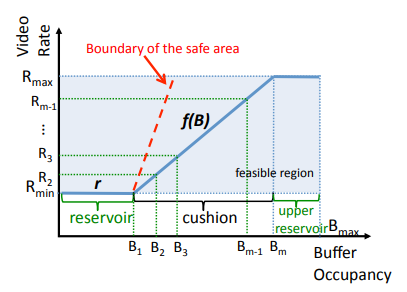
\includegraphics[width=0.5\textwidth]{images/BBA.PNG}
	
	
	
	\caption{The rate-buffer map used in BBA}
	\label {BBA}
	
\end{figure} 
\par To avoid interruption, the client needs to have at least several
segments available in the buffer. The algorithm, therefore, introduces extra intervals: reservoir, cushion, and upper reservoir. When the buffer is filling up the reservoir, the algorithm always request the minimum video bitrate $R_{min}$. Once the reservoir is reached, the client chooses the next bitrate based on the rate-buffer map function $f(B)$ (cushion). When the buffer goes to upper reservoir, the maximum birate $B_{max}$ is chosen.
\par BBA suffers from QoE degradation during
long-term bandwidth fluctuations \cite{ABR cats}.
\subsubsection{BOLA}
BOLA algorithm \cite{BOLA} treats bitrate adaptation as a
utility maximization problem. BOLA defines two performance metrics: \textit{playback utility} $\Bar{v}_N$ representing for quality of playback video and \textit{playback smoothness} $\Bar{s}_N$ that is expected
fraction of time that is spent not rebuffering. The algorithm is designed to maximize the joint utility $\bar{v}_{N}+\gamma\bar{s}_{N}$ where $\gamma$ is an input weight parameter for
prioritizing playback utility versus the playback smoothness.
\par By solving the optimization problem, the optimal solution is to download the next segment at bitrate index $m^{\star}$ where $m^{\star}$ is the index that maximizes the ratio $\rho=(Vv_{m}+V\gamma\tau-b[n])/R_{m}$.
$b[n]$ denotes buffer occupancy in number of segments, which can be calculated by $b[n] = B[n]/\tau$. $v_m$ is the utility of bitrate index $m$, which is non-decreasing function of bitrate. In BOLA, they choose the logarithmic utility function: $v_m=\ln(R_m/R_1)$.  
$V$ is the control parameter which is defined as $V = \cfrac{b_{max}-1}{v_{1}+\gamma\tau}$.
\begin{figure}[!h]
	\centering
	
	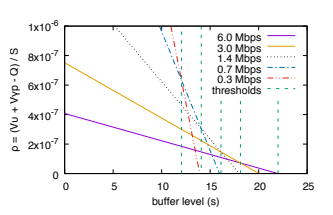
\includegraphics[width=0.5\textwidth]{images/BOLA.PNG}
	
	
	
	\caption{The rate-buffer map used in BOLA}
	\label {BOLA}
	
\end{figure} 
\par As shown in Figure \ref{BOLA}, for each value of buffer occupancy, there is an optimal selection of bitrate that maxmimize the $\rho$ ratio. This scheme somehow is equivalent to rate-buffer map of BBA. The main advantage is that the mapping function is determined with only two parameters $V$ and $\gamma$.
\par So far, BOLA does not uses measured bandwidth to find optimal next segment's bitrate. It can be risky if the algorithm choose a bitrate level that is far bigger than measured bandwidth. Therefore, BOLA defines two schemes to safely switch up to higher bitrate level, which leads to two variants BOLA-U and BOLA-O. BOLA-O mitigates oscillations
by introducing bitrate capping when
switching to a higher bitrate. The segment bitrate is capped at the maximum level that is still smaller than measured bandwidth. The second variant BOLA-U aims to maximize the utility by allowing selected bitrate can reach to the minimum bitrate level that is bigger than measured bandwidth. As the buffer occupancy will decrease when bitrate higher than measured bandwidth, BOLA-U can cause bitrate oscillations.
\section{Proposed Improvements}
In multi-user scenarios, the aforementioned algorithms exhibit some drawbacks in terms of trade-off between efficiency, stability, and fairness. PANDA and FESTIVE are specially designed for multi-user cases. They are equipped with good schemes to perceive the fair-shared bandwidth, therefore, the algorithms achieve good performance in terms of fairness and stability in the steady state. However, due to the discrete nature of bitrate levels, efficiency of bandwidth usage is not high. For example, when two clients compete for the bottleneck of 10 Mbps so that the fair-shared bandwidth each client should receive is around 5 Mbps. Assume there are two bitrate levels of 4 Mbps and 6 Mbps. To maintain the fairness, the algorithms tend to choose the bitrate level of 4 Mbps for both clients, which leads to the waste of 2 Mbps bandwidth.  
\par Buffer-based algorithms such as BOLA can be better than bandwidth-based ones in term of efficiency as they can choose the bitrate levels higher than measured bandwidth. However, they are not designed with dedicated tool to perceived the fair-shared bandwidth. This can cause bitrate fluctuation and unfairness between clients. This is because the fluctuation in measured bandwidth leads to the fluctuation of buffer occupancy, which ends up with fluctuation of bitrate.

\begin{algorithm}
	
	
	\caption{Proposed Algorithm}
	
		
	\For {each time step $n$}
	{
     \nl Estimate the bandwidth share $\hat{x}[n]$ by Equation \ref{BOLA bw}.\\
    
   \nl Produce filtered version $\hat{y}[n]$ by Equation \ref{PANDA smooth}.\\
   \nl $
    	m^{\star}[n]\leftarrow\arg\max_{m}(Vv_{m}+V\gamma\tau-b[n])/R_{m}.$ 
    	\\
    \nl \If{ $m^{\star}[n]>m^{\star}[n-1]$} {
    \nl $m^{\prime}\leftarrow m$ such that $R_{m}<(1-\epsilon)\hat{y}[n]$.\\
    \nl \If{$m^{\prime} < 	m^{\star}[n-1]$}{
       \nl $m^{\star}[n]\leftarrow m^{\star}[n-1]$
    }
   \nl \ElseIf {$m^{\prime}>m^{\star}[n]$}
    {
   \nl \If{$B_[n]<B_{optimal}$}{\nl$m^{\star}[n]\leftarrow m^{\prime}$}.
   \Else{\nl $m^{\star}[n]\leftarrow m^{\prime}+1$} 
    }
    }

\nl Download segment n at bitrate index $m^{\star}[n]$.\\
\nl Schedule the next download as Equation \ref{BOLA buff}.
}
		
\end{algorithm}
\par To address the aforementioned problems of state-of-the-art algorithms, we propose some improvements. The main idea is instead of maintaining the fairness at each time step, we try to keep the fairness in long term. In previous example, where each client tend to choose the same bitrate to achieve the fairness, we give clients the abilities of choosing different bitrate from each other. Specifically, at time step $n$, client 1 can choose the bitrate of 6 Mbps and client 2 choose 4 Mbps. At another time step $n+i$, client 1 will take the bitrate 4 Mbps while the other selects 6 Mbps. In this scheme, the bandwidth of 10 Mbps is fully utilized at each time step and the fairness in the long term is still maintained. We will explain below why the proposed algorithm can achieve this target. 
\par The proposed algorithm presented in Algorithm 3 is a combination of PANDA and BOLA. We take advantages of fair-shared bandwidth estimator and scheduler from PANDA as we consider them well-performed tools in multi-user scenarios. The bitrate selection algorithm is derived from BOLA with some modifications. The algorithm first calculates optimal bitrate index $m^{\star}[n]$ at time step $n$ given by BOLA (line. 3). When switching to higher bitrate, the maximum bitrate index $m^{\prime}$ that is smaller than bandwidth is calculated as a reference. While in BOLA, the reference bitrate is determined by measured bandwidth, here, we use fair-shared bandwidth $\hat{y}[n]$instead as it is more stable. We also introduce $\epsilon$, which controls the safety of algorithm. With larger $\epsilon$, smaller $m^{\prime}$ is chosen.
\par In BOLA, when switching to a bitrate larger than bandwidth, the client always selects the bitrate index $m^{\prime}$ or $m^{\prime}+1$. In our methods, we use the combination of the two options in an online decision. If current buffer occupancy is smaller than optimal buffer level, then we cap the next bitrate under fair-shared bandwidth to avoid bitrate fluctuation (line 10). Otherwise, when buffer is relatively large, we can choose the bitrate larger than fair-shared bandwidth to better exploit the resource (line 11).
\par The propose algorithm can maintain the long-term fairness in multi-user cases. The clients choosing bitrate larger than fair-shared bandwidth will experience buffer decreases, which ends up with switching down bitrate level. Meanwhile, buffer of clients choosing bitrate at level $m^{\prime}$ will increase, which leads to switch up bitrate. This scheme allows clients to achieve the target mentioned in the beginning of this section. Furthermore, by controlling the switching through the optimal buffer level, the algorithm can reduce the frequency of bitrate switches, which guarantees its stability.
\section{Evaluation and Discussion}
% \subsection{Performance metrics}
% In order to evaluate the performance of each algorithm in multi-user cases, we inherit the metrics: instability, inefficiency and unfairness, which are defined in \cite{PANDA}. We only make a  modification to the definition of unfairness in order to evaluate the fairness in the long run.
% \begin{itemize}
% 	\item Instability: The instability of player i at time t is defined as
% 	\begin{equation}
% 	\dfrac{\sum_{d=0}^{k-1}|r_{i,t-d}-r_{i,t-d-1}|\times w(d)}{\sum_{d=0}^{k-1}r_{i,t-d}\times w(d)}
% 	\end{equation}
% 	where $w(d)=k-d$ is weigh function that give more weight for recent samples. k is set to 20 seconds. Generally, this metrics compute the average number of switches with weights over last samples. 
% 	\item Inefficiency: Let C be the available bandwidth.
% 	the inefficiency at time t is defined as
% 	\begin{equation}
% 	\cfrac{\max(0,C-\sum_{i}r_{i,t})}{C}
% 	\end{equation}
% 	\item Unfairness: Let $JainFair$ be the Jain fairness index \cite{JainFair}
% 	calculated on the average bitrate  over all players. The
% 	unfairness is defined as $\sqrt{1 - JainFair}$. Here, we calculate the unfairness in average bitrate of entire video session instead of bitrate at each time step.
% \end{itemize}
\subsection{Experimental setup}
In our experiments, we create a virtual network by Mininet \cite{Mininet} as shown in Figure \ref{Topology}. The network consists of a HTTP Server, and multiple clients, which are connected to the server via two routers. Links between server and Aggregation Router, and between Home Router and HAS Clients are local, which means that they are unbounded and zero delay. We configure the link between two routers to simulate network conditions.
\par 
HTTP Sever and Clients are implemented based on nghttp2 open source. A 400-second video is divided into temporal segments of 2 seconds ($\tau=2s$). Each segment is encoded in 10 different bitrate levels: 459, 693, 937, 1270, 1745, 2536, 3758, 5379,
7861 and 11321 Kbps as in \cite{PANDA}. The buffer size for all algorithms is set to 30s. For fairness, the conventional
player uses the same smoothing and quantizing functions as PANDA as recommended in \cite{PANDA}.
\par Default parameters which are required for implementation of algorithms are listed in Table \ref{parameters}. Each client joins the session at a random time instant and requests the lowest bitrate level for the first video segment in order to quickly fulfill its buffer. 
\begin{figure}[!h]
	\centering
	
	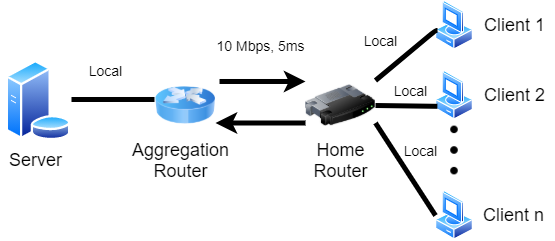
\includegraphics[width=0.5\textwidth]{images/Topology.PNG}
	
	
	
	\caption{Network topology used in simulation.}
	\label {Topology}
	
\end{figure} 

\begin{center}
    

\begin{table}[!h]

    \caption{Parameters used in experiments}
    \label{parameters}
    \centering
	\begin{tabular}{|l|l|c|} 
		\hline
		Algorithm & Parameter & Value \\  
		\hline\hline
		Conventional & $\alpha$ & 0.2\\
		& $\epsilon$ & 0.15 \\
		\hline
		FESTIVE & \textit{targetbuff} & 30s \\ 
		& $\delta$ &12\\
		\hline 
		PANDA & $\alpha$ & 0.2\\
				& $\epsilon$ & 0.15 \\
						& $k$ & 0.14 \\
						& $w$ & 0.3 \\
						& $\beta$ & 0.2 \\
						& $B_{min}$ & 26s\\
		
		
		\hline
		BOLA & $\gamma$ & 2.5\\
		\hline
		Proposed method & $\gamma$ & 2.5\\
		& $\epsilon$ & 0.15 \\
		& $B_{optimal}$ & 28s\\
		\hline
	
	\end{tabular}

\end{table}
\end{center}

\subsection{Experiment results}
First, we consider a system of three clients completing for a bottleneck of 10 Mbps. Figure \ref{Bandwidth comp} shows the estimated shared bandwidth of proposed algorithm and the others. Conventional method in Figure \ref{Bw Conv} and BOLA in Figure \ref{Bw BOLA} simply use measured bandwidth as estimate for the next video segment. Therefore, for both methods, estimated bandwidth experiences many fluctuations over whole session even when the total bandwidth remains unchanged of 10 Mbps. However, the Conventional method fluctuates less frequent than BOLA thanks to applying a filter to smooth out the estimate as shown in Equation 13. The side effect of the filter is to make the magnitude of variations larger. On the other hand, FESTIVE and PANDA as shown in Figure \ref{Bw FESTIVE} and \ref{Bw PANDA}, respectively are specially designed for estimating shared bandwidth in multi-user scenarios. FESTIVE estimates bandwidth by harmonic mean over last 20 samples, which is proved for the robustness against large outliers. Compared to the Conventional and BOLA, this estimation technique can mitigate short-term fluctuations. However, there still exists periodic oscillations in the long term over the session. PANDA exhibits the most accurate estimation, where the estimate of all clients eventually converge to the fair-shared bandwidth and remains at this value over the session. This is because PANDA implements the AIMD mechanism, which is similar to TCP congestion control, to probe the network. Our proposed method inherits the estimation mechanism from PANDA; no fluctuation, therefore, is observed in steady state of the session.
\par Figure \ref{Bitrate comp} illustrates the chosen bitrate at each time step of algorithms over the video session. The chosen bitrate of Conventional algorithm in Figure \ref{Rate Conv} frequently fluctuates over the session due to fluctuations of estimated bandwidth. Despite being a buffer-based algorithm, BOLA still experiences short-term variations in chosen bitrate. This is due to the fact that fluctuations in bandwidth eventually leads to fluctuations in buffer level as formulated in Equation 3.  Another reason is that the estimated bandwidth is also involved in bitrate selection of the algorithm. Besides, those two algorithms do not achieve a good fairness between clients in terms of chosen bitrate. To illustrate, with BOLA algorithm installed, Client 3 always selects lower bitrate than the others. 
\par On the other hand, the chosen bitrate of FESTIVE in Figure \ref{Rate FESTIVE} is in form of periodic square wave with some instant fluctuations. This form is derived from quantizing the sinusoidal periodic waveform of estimated bandwidth. The instant fluctuations are due to the fact that in some certain situations, bitrate selection is extremely sensitive with minor fluctuations of bandwidth. For example, when bandwidth is around 3700 kbps, the client tends to quantize the bandwidth to get the bitrate level of 2536 kbps. However, if the bandwidth increases slightly to 3800 kbps, the client will select another bitrate level, which is 3758 kbps. As shown in Figure \ref{Rate FESTIVE}, most of the time, all clients choose the same bitrate, which proves for good fairness of the algorithm. In terms of efficiency, at some time step, for example at around 130-th second of the session, all clients select the bitrate of 2536 kbps, which is far smaller than fair-allocated bandwidth for each. PANDA in Figure \ref{Rate PANDA} is strictly fair between users in steady state where all clients choose the same bitrate level, which remains unchanged over the session. However, similar to FESTIVE, PANDA does not exhibit good efficiency where all clients do not fully utilize the network resource. 
\par Meanwhile, our proposed algorithm achieves a better trade-off between fairness and efficiency. As shown in Figure \ref{Rate pro}, thanks to the estimation mechanism inherited from PANDA, the Proposed algorithm can precisely perceive fair-shared bandwidth for each user, which results in less fluctuations compared to the Conventional, BOLA and FESTIVE. The instant fluctuations as seen in FESTIVE and BOLA is also removed by using an optimal buffer level to avoid unnecessary switches. Our algorithm is only less stable than PANDA but outperforms PANDA in terms of efficiency where total chosen bitrate at each time step is close to the total bandwidth. 
\begin{figure*}[!h]
	\centering
	
    \begin{subfigure}[t]{0.3\textwidth}
         \centering
         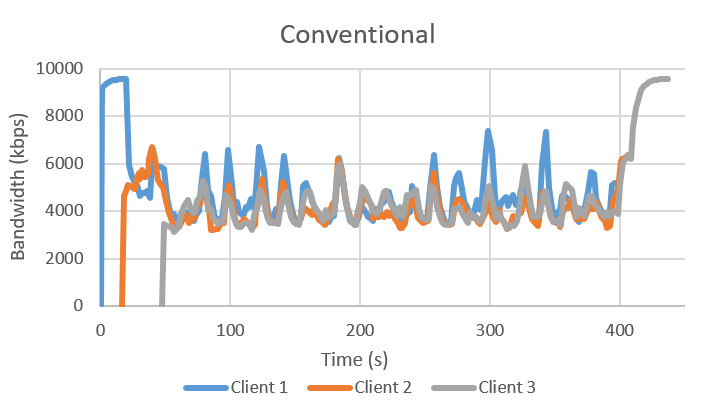
\includegraphics[width=\textwidth]{images/Conventional.png}
         \caption{Conventional algorithm.}
         \label{Bw Conv}
     \end{subfigure}
     \begin{subfigure}[t]{0.3\textwidth}
         \centering
         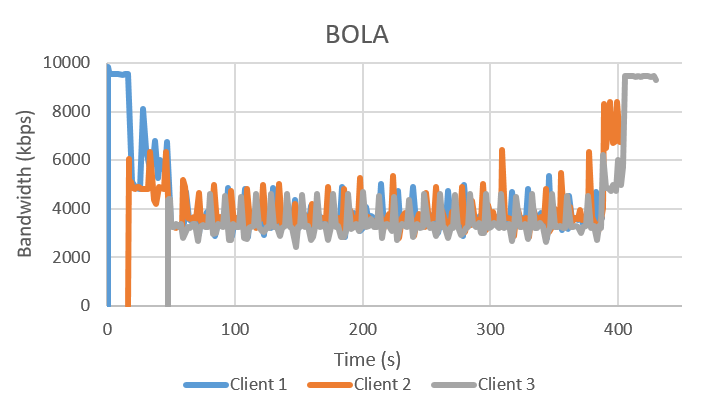
\includegraphics[width=\textwidth]{images/Bw_BOLA.PNG}
         \caption{BOLA}
         \label{Bw BOLA}
     \end{subfigure}
     \\
	\begin{subfigure}[t]{0.3\textwidth}
         \centering
         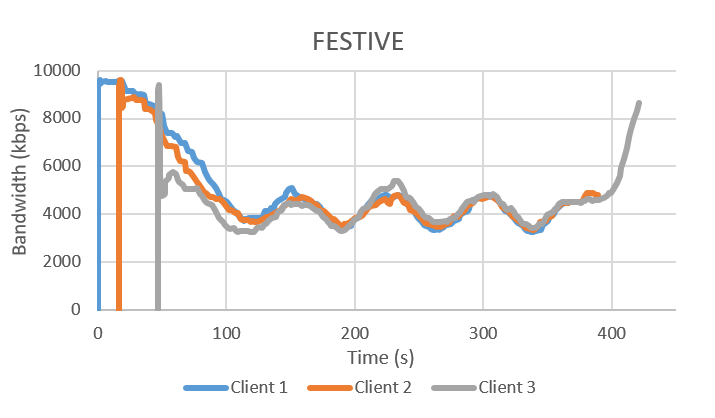
\includegraphics[width=\textwidth]{images/FESTIVE.png}
         \caption{FESTIVE}
         \label{Bw FESTIVE}
     \end{subfigure}
     \begin{subfigure}[t]{0.3\textwidth}
         \centering
         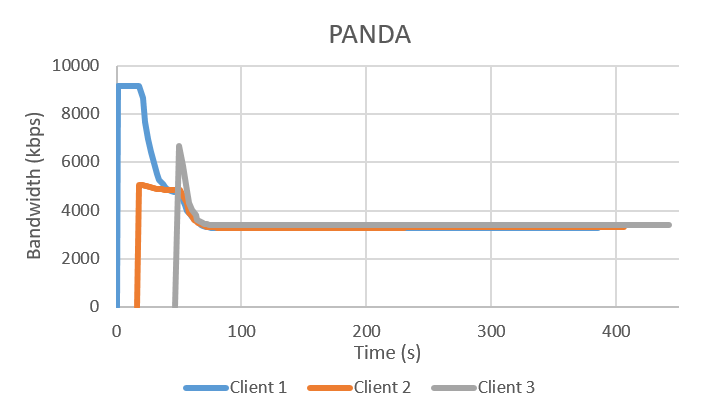
\includegraphics[width=\textwidth]{images/PANDA.PNG}
         \caption{PANDA}
         \label{Bw PANDA}
     \end{subfigure}
	\begin{subfigure}[t]{0.3\textwidth}
         \centering
         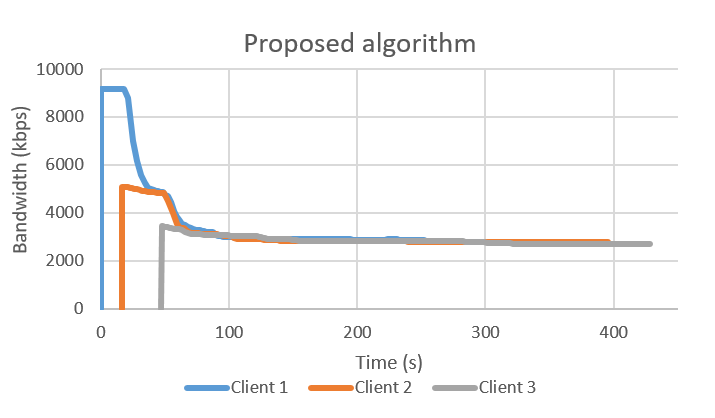
\includegraphics[width=\textwidth]{images/Proposed.png}
         \caption{Proposed algorithm.}
         \label{Bw Pro}
     \end{subfigure}
	
	\caption{Comparison of estimated bandwidth between adaptive algorithms.}
	\label {Bandwidth comp}
	
\end{figure*} 

\begin{figure*}[!h]
	\centering
	
    \begin{subfigure}[t]{0.3\textwidth}
         \centering
         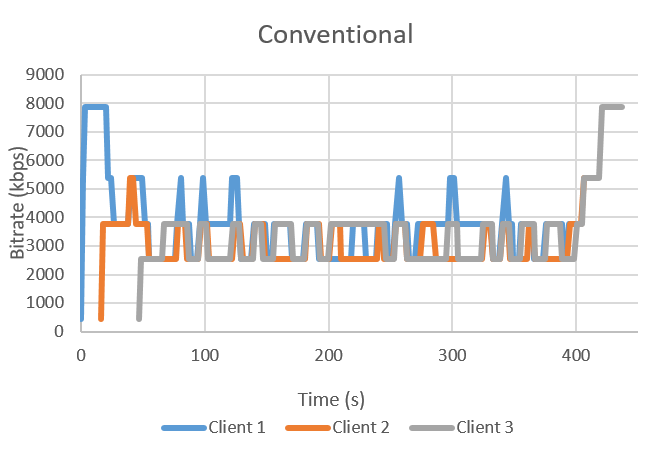
\includegraphics[width=\textwidth]{images/Rate_Conventional.png}
         \caption{Conventional algorithm.}
         \label{Rate Conv}
     \end{subfigure}
     \begin{subfigure}[t]{0.3\textwidth}
         \centering
         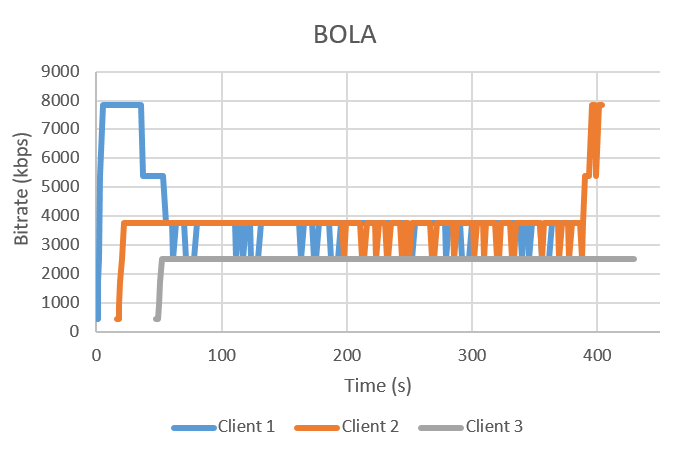
\includegraphics[width=\textwidth]{images/Rate_BOLA.png}
         \caption{BOLA}
         \label{Rate BOLA}
     \end{subfigure}
     \\
	\begin{subfigure}[t]{0.3\textwidth}
         \centering
         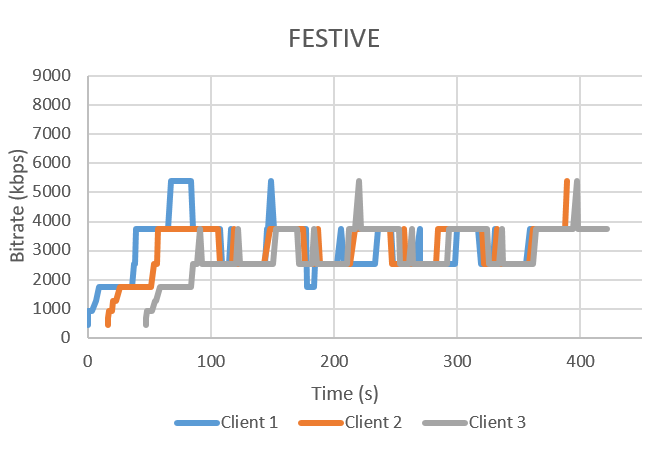
\includegraphics[width=\textwidth]{images/Rate_FESTIVE.png}
         \caption{FESTIVE}
         \label{Rate FESTIVE}
     \end{subfigure}
     \begin{subfigure}[t]{0.3\textwidth}
         \centering
         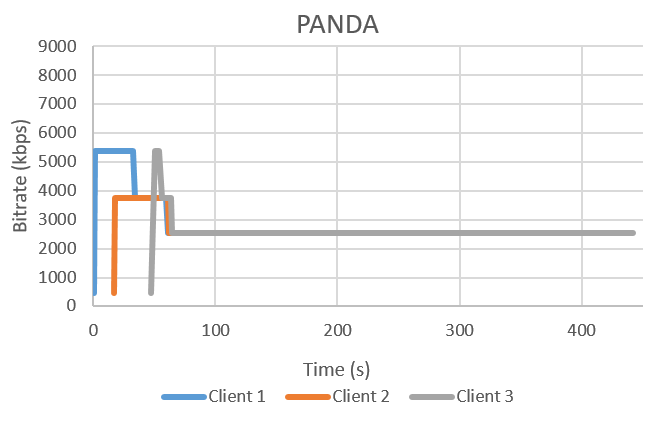
\includegraphics[width=\textwidth]{images/Rate_PANDA.png}
         \caption{BOLA}
         \label{Rate PANDA}
     \end{subfigure}
	\begin{subfigure}[t]{0.3\textwidth}
         \centering
         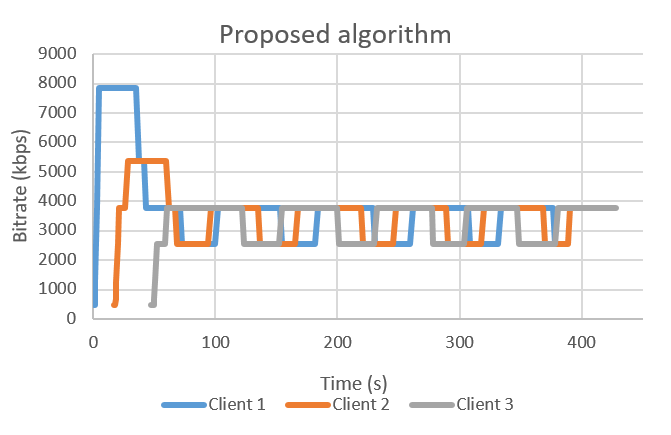
\includegraphics[width=\textwidth]{images/Rate_proposed.png}
         \caption{Proposed algorithm.}
         \label{Rate pro}
     \end{subfigure}
	
	\caption{Comparison of chosen bitrate between adaptive algorithms.}
	\label {Bitrate comp}
	
\end{figure*} 
\begin{figure}[h]
	\centering
	
	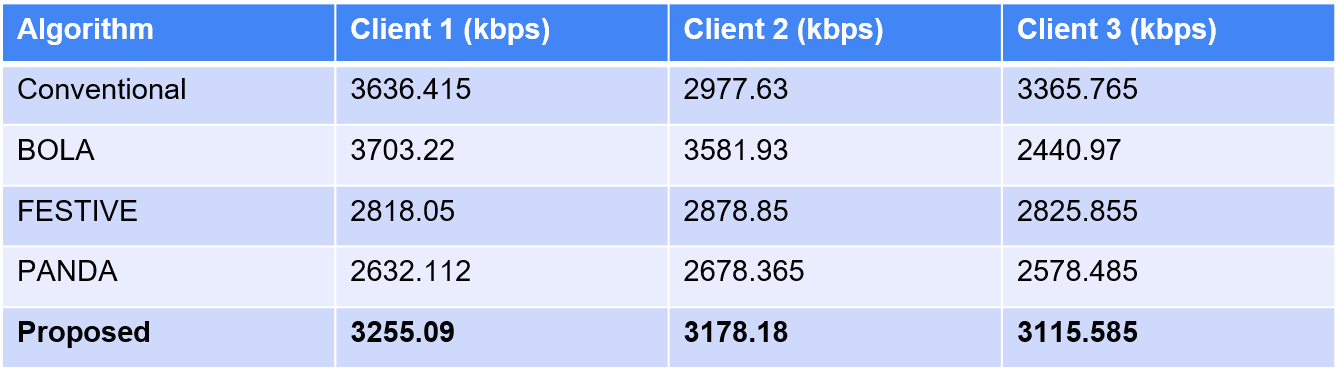
\includegraphics[width=0.5\textwidth]{images/Rate3.png}
	
	
	
	\caption{Average bitrate of 3 users.}
	\label {Rate 3}
	
\end{figure} 
For a clearer comparison, we show in Figure \ref{Rate 3} the average bitrate of each client with each algorithm. The Conventional and BOLA better exploits the network resource where total average bitrate over all clients is almost equal to total bandwidth of 10 Mbps. However, they do not fair between clients. To illustrate, with BOLA installed, the average bitrate of Client 1 and Client 2 (3703 kbps and 
3581 kbps, respectively) are far higher than that of Client 3 with merely 2440 kbps. On the other hand, FESTIVE and BOLA achieve better fairness where all clients witness approximate bitrate values. However, they do not fully utilize the allocated resource where the average bitrate of each client is much smaller than fair-shared bandwidth. The proposed algorithm takes advantages from those two groups. It gives the higher average birate than FESTIVE and PANDA and better fairness between users than the Conventional and BOLA.



\begin{figure}[!h]
	\centering
	
	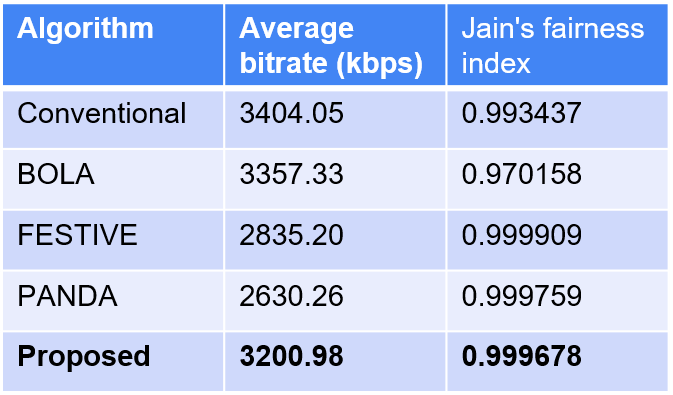
\includegraphics[width=0.4\textwidth]{images/Sum 3.png}
	
	
	
	\caption{Efficiency and Fairness of the algorithms in case of 3 users.}
	\label {Sum 3}
	
\end{figure} 
\begin{figure}[!h]
	\centering
	
	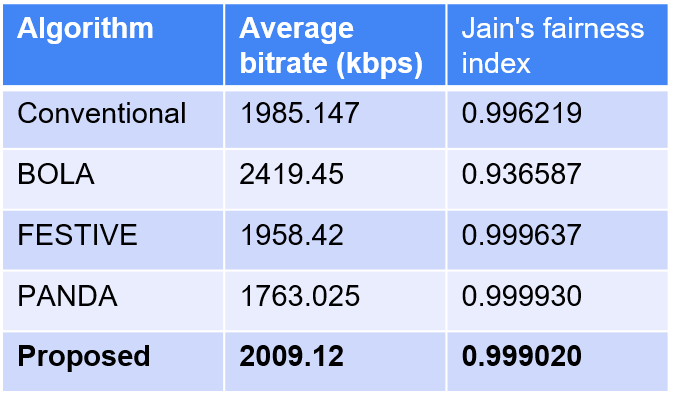
\includegraphics[width=0.4\textwidth]{images/Sum 5.png}
	
	
	
	\caption{Efficiency and Fairness of the algorithms in case of 5 users.}
	\label {Sum 5}
	
\end{figure} 
\par In the second experiment, we extend the system to five clients compete for the bottleneck. We compare the efficiency of the algorithms by the average bitrate over all clients and the fairness by Jain's fairness index as formulated in \cite{JainFair}. The closer the index is to 1, the better the fairness is. Figure \ref{Sum 3} and Figure \ref{Sum 5} show the efficiency and fairness of the algorithms in case of 3 users and 5 users, respectively. In both cases, the proposed algorithm exploits the bandwidth resource more efficiently than FESTIVE and PANDA by getting higher average bitrate over clients. Our algorithm is also much fairer than the Conventional and BOLA but not far away from PANDA and FESTIVE, which is proved by Jain's fairness index.
\section{Conclusions}
While a simple rate adaptation algorithm can perform well with a single client, mutli-user scenarios could lead to unpredictable problems. Two sources of bias have been introduced in this work namely initial condition bias and bitrate selection bias. In this work, we also take a look into two groups of state-of-the-art algorithms and investigate their performance in multi-user scenarios. The first group including the Conventional algorithm, which is widely used in commercial players, and BOLA is not well designed to work with multiple clients. They, despite better exploiting the bandwidth resource, show the poor fairness between clients. On the other hand, FESTIVE and PANDA, which are equipped with effective tools to perceive the shared bandwidth, are fairer in terms of chosen video bitrate between clients. However, they do not efficiently leverage network resource. Our algorithm is proposed to address the problems witnessed in those two groups. We use the same bandwidth estimation mechanism as PANDA and inherit the bitrate selection from BOLA with some improvements for better adaptation in multi-user scenarios. Our algorithm is proved for a better trade-off between efficiency and fairness compared to the reference ones.
% An example of a floating figure using the graphicx package.
% Note that \label must occur AFTER (or within) \caption.
% For figures, \caption should occur after the \includegraphics.
% Note that IEEEtran v1.7 and later has special internal code that
% is designed to preserve the operation of \label within \caption
% even when the captionsoff option is in effect. However, because
% of issues like this, it may be the safest practice to put all your
% \label just after \caption rather than within \caption{}.
%
% Reminder: the "draftcls" or "draftclsnofoot", not "draft", class
% option should be used if it is desired that the figures are to be
% displayed while in draft mode.
%
%\begin{figure}[!t]
%\centering
%\includegraphics[width=2.5in]{myfigure}
% where an .eps filename suffix will be assumed under latex, 
% and a .pdf suffix will be assumed for pdflatex; or what has been declared
% via \DeclareGraphicsExtensions.
%\caption{Simulation results for the network.}
%\label{fig_sim}
%\end{figure}

% Note that the IEEE typically puts floats only at the top, even when this
% results in a large percentage of a column being occupied by floats.


% An example of a double column floating figure using two subfigures.
% (The subfig.sty package must be loaded for this to work.)
% The subfigure \label commands are set within each subfloat command,
% and the \label for the overall figure must come after \caption.
% \hfil is used as a separator to get equal spacing.
% Watch out that the combined width of all the subfigures on a 
% line do not exceed the text width or a line break will occur.
%
%\begin{figure*}[!t]
%\centering
%\subfloat[Case I]{\includegraphics[width=2.5in]{box}%
%\label{fig_first_case}}
%\hfil
%\subfloat[Case II]{\includegraphics[width=2.5in]{box}%
%\label{fig_second_case}}
%\caption{Simulation results for the network.}
%\label{fig_sim}
%\end{figure*}
%
% Note that often IEEE papers with subfigures do not employ subfigure
% captions (using the optional argument to \subfloat[]), but instead will
% reference/describe all of them (a), (b), etc., within the main caption.
% Be aware that for subfig.sty to generate the (a), (b), etc., subfigure
% labels, the optional argument to \subfloat must be present. If a
% subcaption is not desired, just leave its contents blank,
% e.g., \subfloat[].


% An example of a floating table. Note that, for IEEE style tables, the
% \caption command should come BEFORE the table and, given that table
% captions serve much like titles, are usually capitalized except for words
% such as a, an, and, as, at, but, by, for, in, nor, of, on, or, the, to
% and up, which are usually not capitalized unless they are the first or
% last word of the caption. Table text will default to \footnotesize as
% the IEEE normally uses this smaller font for tables.
% The \label must come after \caption as always.
%
%\begin{table}[!t]
%% increase table row spacing, adjust to taste
%\renewcommand{\arraystretch}{1.3}
% if using array.sty, it might be a good idea to tweak the value of
% \extrarowheight as needed to properly center the text within the cells
%\caption{An Example of a Table}
%\label{table_example}
%\centering
%% Some packages, such as MDW tools, offer better commands for making tables
%% than the plain LaTeX2e tabular which is used here.
%\begin{tabular}{|c||c|}
%\hline
%One & Two\\
%\hline
%Three & Four\\
%\hline
%\end{tabular}
%\end{table}


% Note that the IEEE does not put floats in the very first column
% - or typically anywhere on the first page for that matter. Also,
% in-text middle ("here") positioning is typically not used, but it
% is allowed and encouraged for Computer Society conferences (but
% not Computer Society journals). Most IEEE journals/conferences use
% top floats exclusively. 
% Note that, LaTeX2e, unlike IEEE journals/conferences, places
% footnotes above bottom floats. This can be corrected via the
% \fnbelowfloat command of the stfloats package.
% if have a single appendix:
%\appendix[Proof of the Zonklar Equations]
% or
%\appendix  % for no appendix heading
% do not use \section anymore after \appendix, only \section*
% is possibly needed

% use appendices with more than one appendix
% then use \section to start each appendix
% you must declare a \section before using any
% \subsection or using \label (\appendices by itself
% starts a section numbered zero.)
%





% Can use something like this to put references on a page
% by themselves when using endfloat and the captionsoff option.
\ifCLASSOPTIONcaptionsoff
  \newpage
\fi



% trigger a \newpage just before the given reference
% number - used to balance the columns on the last page
% adjust value as needed - may need to be readjusted if
% the document is modified later
%\IEEEtriggeratref{8}
% The "triggered" command can be changed if desired:
%\IEEEtriggercmd{\enlargethispage{-5in}}

% references section

% can use a bibliography generated by BibTeX as a .bbl file
% BibTeX documentation can be easily obtained at:
% http://mirror.ctan.org/biblio/bibtex/contrib/doc/
% The IEEEtran BibTeX style support page is at:
% http://www.michaelshell.org/tex/ieeetran/bibtex/
%\bibliographystyle{IEEEtran}
% argument is your BibTeX string definitions and bibliography database(s)
%\bibliography{IEEEabrv,../bib/paper}
%
% <OR> manually copy in the resultant .bbl file
% set second argument of \begin to the number of references
% (used to reserve space for the reference number labels box)

\begin{thebibliography}{1}

\bibitem{thang}
T. C. Thang, Q.-D. Ho, J.-W. Kang, and A. T. Pham, “Adaptive
Streaming of Audiovisual Content using MPEG DASH,” IEEE Trans.
Consum. Electron., vol. 58, no. 1, pp. 78–85, Feb. 2012
\bibitem{bandwidth fluc}
S. Tullimas, T. Nguyen, R. Edgecomb, and S.-C. Cheung, “Multimedia
streaming using multiple tcp connections,” ACM Trans. Multimedia
Comput. Commun. Appl (ACM TOMCCAP), vol. 4, no. 2, pp. 1–20,
May 2008.
\bibitem{general HTTP} 
A. C. Begen, T. Akgul, and M. Baugher, “Watching video over the web:
Part 2: Applications, standardization, and open issues,” IEEE Internet
Computing, vol. 15, no. 3, pp. 59–63, Apr. 2011
\bibitem{ABR cats}
Abdelhak Bentaleb, Bayan Taani, Ali C. Begen, Christian Timmerer, and Roger
Zimmermann, “A survey on bitrate adaptation schemes for streaming media over HTTP,” IEEE Communications Surveys \& Tutorials, vol. 21, no. 1, pp. 562–585,
2018.
\bibitem{PANDA}
 Z. Li, X. Zhu, J. Gahm, R. Pan, H. Hu, A. C. Begen, and D. Oran,
“Probe and Adapt: Rate Adaptation for HTTP Video Streaming At
Scale,” IEEE Journal on Selected Areas in Communications, vol. 32,
no. 4, pp. 719–733, April 2014.
\bibitem{FESTIVE}
J. Jiang, V. Sekar, and H. Zhang, “Improving Fairness, Efficiency, and
Stability in HTTP-based Adaptive Video Streaming with FESTIVE,”
in Proceedings of the 8th International Conference on Emerging
Networking Experiments and Technologies, ser. CoNEXT ’12. New
York, NY, USA: ACM, 2012, pp. 97–108. 
\bibitem{BBA}
 T.-Y. Huang, R. Johari, N. McKeown, M. Trunnell, and M. Watson,
“A Buffer-based Approach to Rate Adaptation: Evidence from a
Large Video Streaming Service,” SIGCOMM Comput. Commun.
Rev., vol. 44, no. 4, pp. 187–198, Aug. 2014. 

\bibitem{BOLA}
K. Spiteri, R. Urgaonkar, and R. K. Sitaraman, “BOLA: Near-optimal
bitrate adaptation for online videos,” in IEEE INFOCOM 2016 – The
35th Annual IEEE International Conference on Computer Communications, April 2016, pp. 1–9.
\bibitem{Avg rate}
M. Seufert, S. Egger, M. Slanina, T. Zinner, T. Hossfeld,
and P. TranGia, “A Survey on Quality of Experience of
HTTP Adaptive Streaming,” Communications Surveys Tutorials, IEEE, vol. 17, no. 1, pp. 469-492, 2015.
\bibitem{QoE calcu}
Ricky K. P. Mok, Edmond W. W. Chan, and Rocky K. C. Chang,
“Measuring the Quality of Experience of HTTP Video Streaming,” in
IFIP/IEEE International Symposium on Integrated Network Management and Workshops, Dublin, Ireland, May. 2011.
\bibitem{decrease rate}
 R. K. P. Mok, X. Luo, E. W. W. Chan, and R. K. C.
Chang,“ QDASH: A QoE-aware DASH system,” in Proc.
3rd Annu. ACM Conf. MMSys, Chapel Hill, NC, USA. 
\bibitem{liu}  C. Liu, I. Bouazizi, and M. Gabbouj, “Rate Adaptation for
Adaptive HTTP Streaming,” in Proceedings of the Second Annual
ACM Conference on Multimedia Systems, ser. MMSys ’11. New
York, NY, USA: ACM, 2011, pp. 169–174.
\bibitem{Commercial 1} S. Akhshabi, S. Narayanaswamy, Ali C. Begen, and C. Dovrolis. An
experimental evaluation of rate-adaptive video players over HTTP.
Signal Processing: Image Communication, 27:271–287, 2012.
\bibitem{Commercial 2} Te-Yuan Huang, Nikhil Handigol, Brandon Heller, Nick McKeown,
and Ramesh Johari. Confused, timid, and unstable: Picking a video
streaming rate is hard. In Proc. 2012 ACM conference on Internet
measurement, 2012.
\bibitem{Commercial 3}  Chenghao Liu, Imed Bouazizi, and Moncef Gabbouj. Rate Adaptation
for Adaptiv HTTP streaming. In Proc. ACM Multimedia Systems
Conference (MMSys’11), pages 169–174, San Jose, CA, USA, February
2011.
\bibitem{harmonic}
 Harmonic mean.
\url{http://en.wikipedia.org/wiki/Harmonic_mean}
\bibitem{switching}
 N. Cranley, P. Perry, and L. Murphy. User perception of adapting video quality.
International Journal of Human-Computer Studies, 2006.
\bibitem{congestion}
V. Jacobson. Congestion avoidance and control. In Symposium proceedings on Communications architectures and protocols, SIGCOMM ’88,
pages 314–329, New York, NY, USA, 1988. ACM.
\bibitem{BBA}
T.-Y. Huang, R. Johari, N. McKeown, M. Trunnell, and M. Watson,
“A Buffer-based Approach to Rate Adaptation: Evidence from a
Large Video Streaming Service,” SIGCOMM Comput. Commun.
Rev., vol. 44, no. 4, pp. 187–198, Aug. 2014.
\bibitem{BOLA}
K. Spiteri, R. Urgaonkar, and R. K. Sitaraman, “BOLA: Near-optimal
bitrate adaptation for online videos,” in IEEE INFOCOM 2016 – The
35th Annual IEEE International Conference on Computer Communications, April 2016, pp. 1–9.
\bibitem{JainFair}
R. Jain, D. Chiu, and W. Hawe. A quantitative measure of fairness and
discrimination for resource allocation in shared computer system. Technical
Report, DEC, 1984.
\bibitem{Mininet} Mininet \url{http://mininet.org/}
\bibitem{Nghttp2} Nghttp2 \url{https://nghttp2.org/}
\end{thebibliography}

% biography section
% 
% If you have an EPS/PDF photo (graphicx package needed) extra braces are
% needed around the contents of the optional argument to biography to prevent
% the LaTeX parser from getting confused when it sees the complicated
% \includegraphics command within an optional argument. (You could create
% your own custom macro containing the \includegraphics command to make things
% simpler here.)
%\begin{IEEEbiography}[{\includegraphics[width=1in,height=1.25in,clip,keepaspectratio]{mshell}}]{Michael Shell}
% or if you just want to reserve a space for a photo:



% You can push biographies down or up by placing
% a \vfill before or after them. The appropriate
% use of \vfill depends on what kind of text is
% on the last page and whether or not the columns
% are being equalized.

%\vfill

% Can be used to pull up biographies so that the bottom of the last one
% is flush with the other column.
%\enlargethispage{-5in}



% that's all folks
\end{document}


